\begin{figure}[h!]
  \centering
  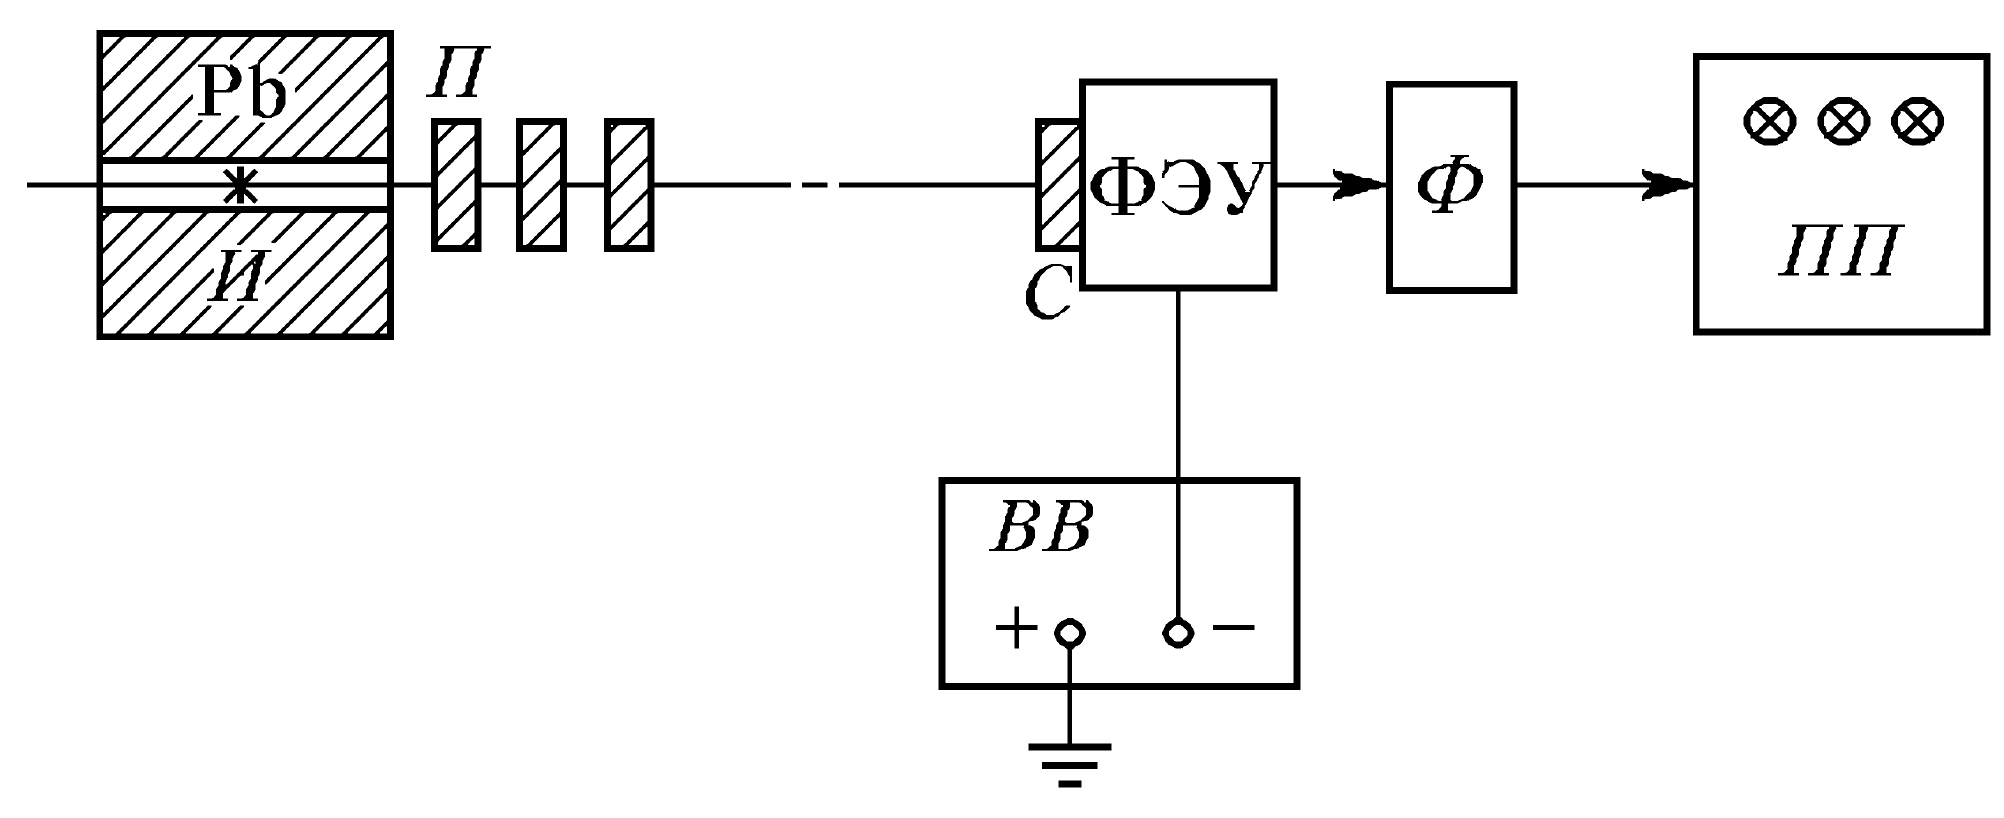
\includegraphics[width=0.7\linewidth]{lab}
  \caption{Блок-схема установки, используемой для измерения коэффициентов
    ослабления потока $\gamma$-лучей: И --- источник $\gamma$-лучей; $Pb$ ---
    свинцовый контейнер с коллиматорным каналом; П --- набор поглотителей; С ---
    сцинтиллятор (кристалл $NaI$($Tl$) ); Ф --- формирователь-выпрямитель}
  \label{ris lab}
\end{figure}

Схема установки, используемой в работе, показана на рис. \ref{ris lab}.
Свинцовый коллиматор выделяет узкий почти параллельный пучок $\gamma$-квантов,
проходящий через набор поглотителей П и регистрируемый сцинтилляционным
счетчиком). Сигналы от счетчика усиливаются и регистрируются пересчетным
прибором ПП. Высоковольтный выпрямитель ВВ обеспечивает питание
сцинтилляционного счетчика.

При недостаточно хорошей геометрии в результаты опытов могут вкрасться
существенные погрешности. В реальных установках всегда имеется конечная
вероятность того, что $\gamma$-квант провзаимодействует в поглотителе несколько
раз до того, как попадет в детектор. Чтобы уменьшить число таких случаев, в
данной работе сцинтилляционный счетчик расположен на большом расстоянии от
источника $\gamma$-квантов, а поглотители имеют небольшие размеры. Их следует
устанавливать за коллиматорной щелью на некотором расстоянии друг от друга,
чтобы испытавшие комптоновское рассеяние и выбывшие из прямого потока кванты с
меньшей вероятностью могли в него вернуться.
